\section{Graph Properties}


A graph is determined by a set of vertices and edges. In the following we will look at some graph properties and features and some definitions of certain graph types. 



%
%
%\begin{definition}{(Empty and Trivial Graphs)}
%A graph \(G = (V,E)\) in which \(V = \varnothing\) is called the empty graph (or null graph).
%A graph in which \(V = \{v\}\) and \(E = \varnothing\) is called the trivial graph.
%\end{definition}
%\begin{definition}{(Isolated Vertex)}\label{def:isver}
%Let \(G = (V,E)\) be a simple graph and let \(v \in V\).
%If \(\deg(v) = 0\) then v is said to be isolated.
%\end{definition}
%%
%\begin{remark}
%Note that Definition~\ref{def:isver} applies only when \(G\) is a simple graph.
%If \(G\) is a general graph (one with self-loops) then \(v\) is still isolated even when \(\{v\} \in E\), that is there is a self-loop at vertex \(v\) and no other edges are adjacent to \(v\).
%In this case, however, \(\deg(v) = 2\).
%\end{remark}
%%
\begin{definition}{(Degree Sequence)}
Let \(G = (V,E)\) be a graph with \(\|V\| = n\).
The degree sequence of \(G\) is a tuple \(d\in \mathbb{Z}^n\) composed of the degrees of the vertices in \(V\) arranged in decreasing order.
\end{definition}
%
\begin{example}
Consider the graph in Figure~\ref{fig:g3}.
The degrees for the vertices of this graph are:
\[v_1 = 4 \quad v_2 = 3 \quad v_3 = 2 \quad v_4 = 2 \quad v_5 = 1\]
This leads to the degree sequence: \(d = (4, 3, 2, 2, 1)\).
\end{example}
%
\begin{figure}
\centering
\begin{tikzpicture}[nodestyle/.style={draw,shape=circle, fill=white, blur shadow={shadow blur steps=5}},]
  % put nodes at the corners of a pentagon
  \node[regular polygon,regular polygon sides=5,minimum size=3.5cm, shape border rotate=20] (p) {};
  \foreach\x/\y in {1/1,2/4,3/3,4/5,5/2}{
    % name nodes accordingly
    \node[nodestyle] (p\y) at (p.corner \x){\y};
  }
  % draw edges
  \draw (p1) -- (p2);
  \draw (p1) -- (p3);
  \draw (p1) -- (p4);
  \draw (p1) -- (p5);
  \draw (p2) -- (p3);
  \draw (p2) -- (p4);
\end{tikzpicture}
\caption{\label{fig:g3}%
The graph above has a degree sequence \(d = (4; 3; 2; 2; 1)\).
These are the degrees of the vertices in the graph arranged in decreasing order.
}
\end{figure}
%


\begin{remark} (Pigeonhole principle).
Suppose items may be classified according to \(m\) possible types and we are given \(n> m\) items.
Then there are at least two items with the same type.
This Pigeonhole principle was originally formulated by thinking of placing \(m + 1\) pigeons into \(m\) pigeon holes.
Clearly to place all the pigeons in the holes, one hole has two pigeons in it.
The holes are the types (each whole is a different type) and the pigeons are the items.

\end{remark}
%
\begin{theorem}
Let \(G = (V, E)\) be a non-empty, non-trivial graph.
Then \(G\) has at least one pair of vertices with equal degree.
\end{theorem}
%
\begin{proof}
This proof uses the Pigeonhole principle and is illustrated by the graph in Figure~\ref{fig:g3}, where \(\deg(v_3) = \deg(v_4)\).
The types will be the possible vertex degree values and the objects will be the vertices.

Suppose  \(|V| = n\).
Each vertex could have a degree between \(0\) and \(n-1\) (for a total of \(n\) possible degrees), but if the graph has a vertex of degree \(0\) then it cannot have a vertex of degree \(n-1\).
Therefore, there are only at most \(n-1\) possible degree values depending on whether the graph has an isolated vertex or a vertex with degree \(n-1\) (if it has neither, there are even fewer than \(n-1\) possible degree values).
Thus by the Pigeonhole Principle, at least two vertices must have the same degree.
\end{proof}
%
\begin{definition}{(Graphic Sequence)}
Let \(d = (d_1, \ldots, d_n)\) be a tuple in \(\mathbb{Z}^n\) with \(d_1 \geq d_2 \geq \cdots \geq d_n\).
Then \(d\) is graphic if there exists a graph \(G\) with degree sequence \(d\).
\end{definition}
%
\begin{corollary}
If d is graphic, then the sum of its elements is even.
\end{corollary}
%
\begin{proof}
This follows from Theorem~\ref{thm:deg}.
\end{proof}
%


\subsection{Special Graphs}
\begin{definition} {(Complete Graph)}
Let \(G = (V,E)\) be a graph with \(|V| = n\) with \(n \geq 1\).
If the degree sequence of \(G\) is \((n-1,n-1,\dots,n-1) \) then \(G\) is called a complete graph on \(n\) vertices and is denoted \(K_n\).
In a complete graph on \(n\) vertices each vertex is connected to every other vertex by an edge.
\end{definition}

\begin{lemma}
Let \(K_n = (V, E)\) be the complete graph on \(n\) vertices.
Then: \(|E| = \frac{n(n-1)}{2}\).
\end{lemma}
%
\begin{corollary}
Let \(G = (V, E)\) be a graph and let \(|V | = n\).
Then:
\[0\leq |E|\leq  \begin{pmatrix}n\\2\end{pmatrix}.\]
\end{corollary}

\begin{definition}{(Regular Graph)}
Let \(G = (V,E)\) be a graph with \(|V| = n\).
If the degree sequence of \(G\) is \((k, k,\ldots, k)\) with \(k \leq n-1\) then \(G\) is called a \(k\)-regular graph on \(n\) vertices.
\end{definition}
%


%
\begin{figure}
  \centering
  \begin{subfigure}[b]{0.32\textwidth}
    \centering
    \begin{tikzpicture}[baseline, nodestyle/.style={node font=\tiny, shape=circle, fill=yellow}]
  % put nodes at the corners of a triangle
  \node[regular polygon,regular polygon sides=3,minimum size=5cm] (p) {};
  % nodes at corners
  \foreach\x/\y in {1/2,2/4,3/3}{\node[nodestyle] (p\y) at (p.corner \x){\y};}
  % node at centroid
  \node[nodestyle] (p1) at (p.center) {1};
  % draw edges
  \graph[edges=blue]{
    \foreach\x in {1,2,3}{
      \foreach\y in {\x,...,4}{
        (p\x) -- (p\y);
      }
    }
  };
\end{tikzpicture}
    \caption{\(K_4\)}\label{fig:graph4a}
  \end{subfigure}
  \begin{subfigure}[b]{0.32\textwidth}
    \centering
    % Modified from https://tex.stackexchange.com/a/625537
\begin{tikzpicture}[
  baseline,
  every node/.style={node font=\tiny, shape=circle, fill=yellow, inner sep=1pt, minimum size=2pt},
  every edge/.style={draw=blue}
]
  \graph[math nodes, clockwise] {
      subgraph I_n [V={6,9,7,10,8}] --
      subgraph C_n [V={1,2,3,4,5},radius=1.23cm];
      {[cycle] 6,7,8,9,10}
    };
\end{tikzpicture}
    \caption{Petersen Graph}\label{fig:graph4b}
  \end{subfigure}
  \begin{subfigure}[b]{0.32\textwidth}
    \centering
    % Modified from: https://www.integral-domain.org/lwilliams/Resources/TikzImg/dodecagraph.tex

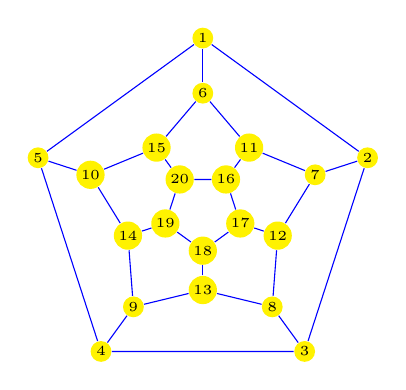
\begin{tikzpicture}[
  baseline,
  every node/.style = {
    circle,
    fill=yellow,
    node font=\tiny,
    inner sep=1pt,
    minimum size=2pt
  },
  uedge/.style={draw=blue}
]
    \foreach \x [
      evaluate=\x as \xo using {int(mod(6-\x,5)+1)},
      evaluate=\x as \xi using {int(mod(6-\x,5)+6)},
      evaluate=\x as \xii using {int(mod(5-\x,5)+11)},
      evaluate=\x as \xiii using {int(mod(5-\x,5)+16)},
    ] in {0,1,2,3,4}{
        \node (o\x) at (18+\x*72:2.2cm) {\xo};
        \node (i\x) at (18+\x*72:1.5cm) {\xi};
        \node (ii\x) at (54+\x*72:1cm) {\xii};
        \node (iii\x) at (54+\x*72:0.5cm) {\xiii};
    }
    \foreach \x in {0,1,2,3,4}{
        \path[uedge] (o\x) edge (i\x);
        \path[uedge] (ii\x) edge (iii\x);
    }
    \path[uedge] (o0)--(o1)--(o2)--(o3)--(o4)--(o0);
    \path[uedge] (iii0)--(iii1)--(iii2)--(iii3)--(iii4)--(iii0);
    \path[uedge] (i0)--(ii0)--(i1)--(ii1)--(i2)--(ii2)--(i3)--(ii3)--(i4)--(ii4)--(i0);
\end{tikzpicture}
    \caption{Dodecahedron}\label{fig:graph4c}
  \end{subfigure}
  \caption{This are three examples of 3-regular graphs, where $K_4$ (a) is a complete graph but the others are not. The Peterson Graph (b) is a 3-regular graph that is used in many graph theoretic examples. The dodecahedron (c) really is a flattened dodecahedron, one of the five platonic solids from classical geometry.}\label{fig:graph4}
\end{figure}
%
\subsection{Directed Graphs}
%
\begin{definition}{(Directed Graph)}
A directed graph (digraph) is a tuple \(G = (V,E)\) where \(V\) is a (finite) set of vertices and \(E\) is a collection of elements contained in \(V \times V\).
That is, \(E\) is a collection of ordered pairs of vertices.
The edges in \(E\) are called directed edges to distinguish them from those edges in Definition~\ref{def:graph}.
\end{definition}
%
\begin{definition}{(Source / Destination)}
Let \(G = (V,E)\) be a directed graph.
The source (or tail) of the (directed) edge \(e = (v_1,v_2)\) is \(v_1\) while the destination (or sink or head) of the edge is \(v_2\).
\end{definition}
%
\begin{remark}
A directed graph (digraph) differs from a graph only insofar as we replace the concept of an edge as a set with the idea that an edge as an ordered pair in which the ordering gives some notion of direction of flow.
In the context of a digraph, a self-loop is an ordered pair with form \((v,v)\).
We can define a multi-digraph if we allow the set \(E\) to be a true collection (rather than a set) that contains multiple copies of an ordered pair.
\end{remark}
%
\begin{remark}
It is worth noting that the ordered pair \((v_1,v_2)\) is distinct from the pair \((v_2, v_1)\).
Thus if a digraph \(G = (V, E)\) has both \((v_1, v_2)\) and \((v_2, v_1)\) in its edge set, it is not a multi-digraph.
\end{remark}
%
\begin{example}
We can modify the figures in Example~\ref{ex1} to make it directed.
Suppose we have the directed graph with vertex set \(V = \{1, 2, 3, 4\}\) and edge set: \(E = \{(1, 2),\allowbreak (2, 3),\allowbreak (3, 4),\allowbreak (4, 1)\}\).
This digraph is visualized in Figure~\ref{fig:gr2-a}.
In drawing a digraph, we simply append arrow- heads to the destination associated with a directed edge.
We can likewise modify our self-loop example to make it directed.
In this case, our edge set becomes: \(E = \{(1, 2),\allowbreak (2, 3),\allowbreak (3, 4),\allowbreak (4, 1),\allowbreak (1, 1)\}\).
This is shown in Figure~\ref{fig:gr2-b}.
\end{example}
%
\begin{figure}
\centering
\begin{subfigure}[b]{0.49\textwidth}
  \centering
  \begin{tikzpicture}[>={Stealth[round]}, semithick]
  \graph [%
    simple necklace layout, nodes={ draw, circle, node sep=2cm}
  ] {%
    1 -> [orient=0]  2 -> 3 -> 4 -> 1%
  };
\end{tikzpicture}
  \caption{\label{fig:gr2-a}}%
\end{subfigure}
\begin{subfigure}[b]{0.49\textwidth}
  \centering
  \tikzset{every loop/.style={in=60,out=120}}
\begin{tikzpicture}[>={Stealth[round]}, semithick]
  \graph [%
    simple necklace layout, nodes={ draw, circle, node sep=2cm}
  ] {%
    1 -> [orient=0]  2 -> 3 -> 4 -> 1 -> [loop left] 1 %
  };
\end{tikzpicture}
  \caption{\label{fig:gr2-b}}%
\end{subfigure}
\caption{
(a) A directed graph.
(b) A directed graph with a self-loop.
In a directed graph, edges are directed; that is they are ordered pairs of elements drawn from the vertex set.
The ordering of the pair gives the direction of the edge.
}
\end{figure}
%
\begin{definition}{(Underlying Graph)}
If \(G = (V,E)\) is a digraph, then the underlying graph of G is the (multi) graph (with self-loops) that results when each directed edge \((v_1, v_2)\) is replaced by the set \(\{v_1, v_2\}\) thus making the edge non-directional.
Naturally if the directed edge is a directed self-loop \((v, v)\) then it is replaced by the singleton set \({v}\).
\end{definition}
%
\begin{remark}
Notions like edge and vertex adjacency and neighborhood can be extended to digraphs by simply defining them with respect to the underlying graph of a digraph.
Thus the neighborhood of a vertex \(v\) in a digraph \(G\) is \(N(v)\) computed in the underlying graph.
\end{remark}
%
\begin{remark}
Whether the underlying graph of a digraph is a multi-graph or not usually has no bearing on relevant properties.
In general, an author will state whether two directed edges \((v_1, v_2\)) and \((v_2, v_1)\) are combined into a single set \(\{v_1, v_2\}\) or two sets in a multiset.
As a rule-of-thumb, multi-digraphs will have underlying multigraphs, while digraphs generally have underlying graphs that are not multi-graphs.
\end{remark}
%
\begin{remark}
It is possible to mix (undirected) edges and directed edges together into a very general definition of a graph with both undirected and directed edges.
Situations requiring such a model almost never occur in modeling and when they do, the undirected edges with form \(\{v_1, v_2\}\) are usually replaced with a pair of directed edges \((v_1, v_2)\) and \((v_2, v_1)\).
Thus, for remainder of these notes, unless otherwise stated:
\begin{enumerate}
\item When we say `graph', we will mean simple graph as in Remark~\ref{rem:simple}.
If we intend the result to apply to any graph we’ll say a general graph.
\item When we say `digraph', we will mean a directed graph \(G = (V, E)\) in which every edge is a directed edge and the component \(E\) is a set and in which there are no self-loops.
\end{enumerate}
\end{remark}
\begin{definition}{(In-Degree, Out-Degree)}
Let \(G = (V, E)\) be a digraph.
The in-degree of a vertex \(v\) in \(G\) is the total number of edges in \(E\) with destination \(v\).
The out-degree of \(v\) is the total number of edges in \(E\) with source \(v\).
We will denote the in-degree of \(v\) by \(\deg_{in}(v)\) and the out-degree by \(\deg_{out}(v)\).
\end{definition}

\begin{theorem}
Let \(G = (V, E)\) be a digraph.
Then the following holds:
\begin{equation}
|E| =\sum_{v\in V} \deg_{in}(v) =\sum_{v\in V} \deg_{out}(v).
\end{equation}
\end{theorem}

\subsection{Subgraphs}
%
\begin{definition}{(Subgraph)}
Let \(G = (V, E)\).
A graph \(H = (V', E')\) is a subgraph of \(G\) if \(V' \subseteq V\) and \(E'\subseteq E\).
The subgraph \(H\) is proper if \(V' \subsetneq V\) or \(E' \subsetneq E\).
\end{definition}
%
\begin{example}%
We illustrate the notion of a sub-graph in Figure~\ref{fig:subg}.
Here we illustrate a sub-graph of the Petersen Graph.
The sub-graph contains vertices 6, 7, 8, 9 and 10 and the edges connecting them.
\end{example}
%
\begin{definition}{(Spanning Subgraph)}
Let \(G = (V, E)\) be a graph and \(H = (V', E') \) be a subgraph of \(G\).
The subgraph \(H\) is a spanning subgraph of \(G\) if \(V' = V\).
\end{definition}

\begin{figure}
  \centering
  \begin{subfigure}{0.32\textwidth}
    \centering
    % Modified from https://tex.stackexchange.com/a/625537
\begin{tikzpicture}[
  baseline,
  every node/.style={node font=\tiny, shape=circle, fill=yellow, inner sep=1pt, minimum size=2pt},
  every edge/.style={draw=blue}
]
  \graph[math nodes, clockwise] {
      subgraph I_n [V={6,9,7,10,8}] --
      subgraph C_n [V={1,2,3,4,5},radius=1.23cm];
      {[cycle] 6,7,8,9,10}
    };
\end{tikzpicture}
    \caption{Petersen Graph}
  \end{subfigure}
  \begin{subfigure}{0.32\textwidth}
    \centering
    % Modified from https://tex.stackexchange.com/a/625537
\begin{tikzpicture}[
  every node/.style={node font=\tiny, shape=circle, fill=yellow},
  every edge/.style={draw=blue}
]
  \graph[math nodes, clockwise, edge=red] {
      subgraph I_n [V={6,9,7,10,8}, nodes={fill=green}] -- [edges=blue]
      subgraph C_n [V={1,2,3,4,5},radius=1.25cm, edge=blue];
      {[cycle] 6,7,8,9,10}
    };
\end{tikzpicture}
    \caption{Highlighted Subgraph}
  \end{subfigure}
  \begin{subfigure}{0.32\textwidth}
    \centering
    \begin{tikzpicture}[
  every node/.style={node font=\tiny, shape=circle, fill=yellow},
  every edge/.style={draw=blue}
]
\graph [clockwise] { subgraph C_n [V={6,...,10}, radius=2.2cm] };
\end{tikzpicture}
    \caption{Extracted Subgraph}
  \end{subfigure}
  \caption{\label{fig:subg}%
The Petersen Graph is shown (a) with a sub-graph highlighted (b) and that sub-graph displayed on its own (c).
A sub-graph of a graph is another graph whose vertices and edges are sub-collections of those of the original graph.
}%
\end{figure}
%
%\begin{definition}{(Edge Induced Subgraph)}
%Let \(G = (V, E)\) be a graph.
%If \(E'\subseteq E\).
%The subgraph of \(G\) induced by \(E'\) is the graph \(H=(V',E')\)
%where \(v\in V'\) if and only if \(v\) appears in an edge in \(E\).
%\end{definition}
%%
%\begin{definition}{ (Vertex Induced Subgraph)}
%Let \(G = (V, E)\) be a graph.
%If \(V'\subseteq V\), the subgraph of \(G\) induced by \(V'\) is the graph \(H=(V',E')\) where \({v_1,v_2}\in E'\) if and only if \(v_1\) and \(v_2\) are both in \(V'\).
%\end{definition}
%
\begin{remark}
For directed graphs, all sub-graph definitions are modified in the obvious way.
Edges become directed as one would expect.
\end{remark}
